\documentclass[mathserif]{beamer} 
\usepackage{eulervm} %красивый математический шрифт - по желанию
\usepackage{ulem} %зачёркивания
\usepackage{bm} %особо жирный математический
\usepackage{schemata} %для красивых блочных переходов, пользуюсь редко
\usepackage{mathtools} %улучшенная работа с типографией в math mode
\setbeamertemplate{navigation symbols}{} %отключает управляющие символы в правом нижнем углу
\usefonttheme{professionalfonts}
\usepackage{cmap} %чтобы были работающие гиперссылки
\usepackage{makeidx,fancybox,tikz}
\usetikzlibrary{automata, positioning, arrows,patterns}
\usetikzlibrary{arrows.meta}
\usepackage{tempora} %по желанию -- русские штрифты с засечками

\mode<presentation>
{
% \usetheme{Warsaw}
%  \usetheme{Frankfurt}
%  \usetheme{Singapore}
%  \usetheme{Boadilla}
%  \usetheme{Montpellier}
%  \usetheme{Szeged}
  \usetheme{CambridgeUS} %тут решайте сами, что выбрать
    % or ...

%  \usecolortheme{dolphin}
  \usecolortheme{dove} %аналогично
%  \usecolortheme{wolverine}
%  \usecolortheme{crane}

%  \usefonttheme{structurebold}
%  \usefonttheme{structuresmallcapsserif}

%  \setbeamercovered{transparent}
}
\usepackage[T1,T2A]{fontenc}
\usepackage[utf8]{inputenc}
\usepackage[english,russian]{babel}
\usepackage{amsmath,mathrsfs} %ещё больше математических символов
\usepackage{amstext}
\usepackage{graphicx,relsize}
% \usepackage{graphicx}
\graphicspath{ {./documentation/} }

\usepackage{color}
\definecolor{gray}{rgb}{0.4,.4,0.4} %здесь можно определить собственные цвета
\definecolor{grey80}{rgb}{0.8,.8,0.8}
\definecolor{grey90}{rgb}{0.9,.9,0.9}
\definecolor{grey95}{rgb}{0.95,.95,0.95}
\newcommand\redstroke{\bgroup\markoverwith
{\textcolor{red}{\rule[0.5ex]{2pt}{1.5pt}}}\ULon} %зачёркивание жирной красной чертой

\newcommand\reduline{\bgroup\markoverwith
{\textcolor{red}{\rule[-0.5ex]{2pt}{1.5pt}}}\ULon}%подчёркивание жирной красной чертой

\newcommand\bluline{\bgroup\markoverwith
{\textcolor{blue}{\rule[-0.5ex]{2pt}{1.5pt}}}\ULon}

\newcommand\bolduline{\bgroup\markoverwith
{\textcolor{white}{\rule[-0.5ex]{2pt}{1.5pt}}}\ULon}

\title[] {Автомат Томпсона}

\author[Chipollino]{Лучшая команда разработчиков по ТФЯ} % :))
\date[] 
{2022 г.}
\subject{Computer Science}

\newcommand{\Lang}{\mathscr{L}} %макрос для языка регулярки или автомата
\def\logor{\mathrel{\vee}} %отрендеренные логические операторы (с правильными интервалами)
\def\logimpl{\mathrel{\Rightarrow}}
\def\Linearize{\mathtt{Linearize}} %названия операций интерпретатора записываем моноширинным
\def\First{\mathrm{First}} %названия прочих операций записываем обычным шрифтом, но не тем, который в math mode по умолчанию
\def\Last{\mathrm{Last}}
\def\Follow{\mathrm{Follow}}
\def\Glushkov{\mathtt{Glushkov}}
\def\Thompson{\mathtt{Thompson}}
\def\logand{\mathrel{\&}}
\def\lognot{\mathop{\neg}}
\def\iff{\mathrel{\Leftrightarrow}}
\def\quantall#1{\mathop{\forall #1}}
\def\quantex#1{\mathop{\exists #1}} 
\def\alter{\ensuremath{\mathrel{\vert}}}%отрендеренные регулярные операторы 
\def\star{\ensuremath{^{*}}}%отрендеренные регулярные операторы 
\def\regexpstr#1{\mathtt{#1}}%буквы внутри регулярок переписываются в моноширинный
\newcommand{\Nat}{\mathbb N}
\newcommand{\empt}{\varepsilon} %пустое слово
\newcommand{\bottom}{\bot} %противоречие
\newcommand{\rar}{\rightarrow} %стрелка вправо. Для экономии букв.
\newcommand{\RegExp}{\mathcal{RE}} %макрос для обозначения множества всех регулярок
%в преамбулу можно и нужно добавлять свои макросы

\begin{document}

\maketitle
\section{Основные понятия}
\begin{frame}{Адгоритм Томпсона и НКА}
    \begin{block}{\bf Основные сведения}
        В информатике алгоритм построения Томпсона представляет собой метод преобразования регулярного выражения в эквивалентный недетерминированный конечный автомат (НКА). Этот НКА можно использовать для сопоставления строк с регулярным выражением.
        Регулярные выражения и недетерминированные конечные автоматы - это два представления формальных языков.
    \end{block}
\end{frame}% descriptive documentation
\begin{frame}{НКА}
    \vspace{-5pt}
    \begin{block}{\bf Определение}
        Недетерминированный конечный автомат (НКА) -- это детерминированный конечный автомат (ДКА), который не выполняет следующие условия:
        \begin{itemize}
            \item любой его переход единственным образом определяется по текущему состоянию и входному символу;
            \item чтение входного символа требуется для каждого изменения состояния.
        \end{itemize}
    \end{block}
    % \begin{exampleblock}{\bf Пример}
    %     НКА:

    %     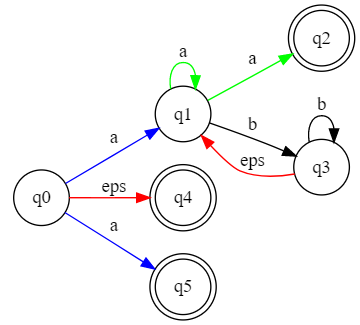
\includegraphics[width=2in, keepaspectratio]{tompson1.png}
    % \end{exampleblock}
\end{frame}% descriptive documentation
\begin{frame}{НКА}
    \begin{block}{\bf Определение}
        НКА формально представляется как 5-кортеж $(Q,\Sigma ,\Delta ,q_{0},F)$, состоящий из:
        \begin{itemize}
            \item конечного множества состояний $Q$.
            \item конечного множества входных символов $\Sigma$.
            \item функции переходов $\Delta$  :  $Q\times \Sigma \rightarrow P(Q)$.
            \item начального состояния $q_{0}\in Q$.
            \item множества состояний $F$ распознаваемых как конечные состояния  $F\subseteq Q$.
        \end{itemize}
        Здесь $P(Q)$ означает степень множества $Q$.
    \end{block}
\end{frame}% descriptive documentation

\section{Автомат Томпсона}
\begin{frame}{Конструкция автомата Томпсона}
    \vspace{-5pt}
    \begin{block}{\bf Алгоритм построения $\Thompson(r)$}
        Алгоритм работает рекурсивно, разбивая выражение на составляющие его подвыражения, из которых будет построен НКА с использованием набора правил. Точнее, из регулярного выражения $R$ полученный автомат $A$ с переходной функцией $\Delta$ учитывает следующие свойства:
        \begin{itemize}
            \item $A$ имеет ровно одно начальное состояние $q_{0}$, которое недоступно ни из какого другого состояния. То есть для любого состояния $q$ и любой буквы $a$ $\Delta (q,a)$ не содержит $q_{0}$.
            \item $A$ имеет ровно одно конечное состояние $q_{f}$, которое недоступно ни из какого другого состояния. То есть для любой буквы $а$, $\Delta (q_{f},a)=\emptyset$.
            \item Пусть $c$ - число конкатенаций регулярного выражения $R$, а $s$ — количество символов, не считая круглых скобок, то есть $\alter, \star, a, \empt$. Тогда число состояний $A$ равно $2s - c$ (линейно по размеру $R$).
            \item Число переходов, выходящих из любого состояния, не более двух.
            \item Поскольку НКА из $m$ состояний и не более $e$ переходов из каждого состояния может соответствовать строке длиной $n$ за время $O(emn)$, НКА Томпсона может выполнять сопоставление с образцом за линейное время, предполагая алфавит фиксированного размера.
        \end{itemize}
    \end{block}
\end{frame} % descriptive documentation

\begin{frame}{Правила}
    \vspace{-5pt}
    \begin{block}{\bf }
        Пустое выражение $\empt$ преобразуется в\\
        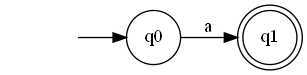
\includegraphics[width=2in, keepaspectratio]{tompson_rule2.png}

        Символ $a$ входного алфавита преобразуется в\\
        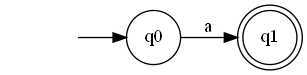
\includegraphics[width=2in, keepaspectratio]{tompson_rule2.png}

        Выражение объединения $s\alter t$ преобразуется в\\
        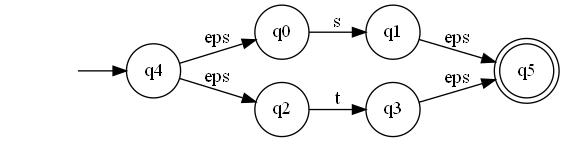
\includegraphics[width=2in, keepaspectratio]{tompson_rule3.png}\\
        Состояние $q_{4}$ переходит через $\empt$ либо в начальное состояние $N(s)$, либо $N(t)$. Их конечные состояния становятся промежуточными состояниями всего НКА и сливаются через два $\empt$-перехода в конечное состояние НКА.
    \end{block}
\end{frame}% descriptive documentation
\begin{frame}{Правила}
    \vspace{-5pt}
    \begin{block}{\bf }
        Выражение конкатенации $st$ преобразуется в\\
        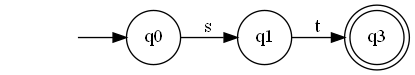
\includegraphics[width=2in, keepaspectratio]{tompson_rule4.png}\\
        Начальное состояние $N(s)$ является начальным состоянием всего НКА. Конечное состояние $N(s)$ становится начальным состоянием $N(t)$. Конечное состояние $N(t)$ является конечным состоянием всего НКА.

        Выражение Клини Стар $s\star$ преобразуется в\\
        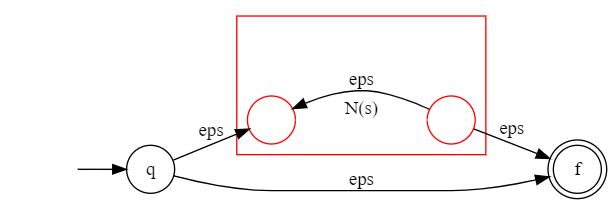
\includegraphics[width=2in, keepaspectratio]{tompson_rule5.png}\\
        $\empt$-переход соединяет начальное и конечное состояние НКА с промежуточным НКА $N(s)$. Другой $\empt$-переход от внутреннего конечного к внутреннему начальному состоянию $N(s)$ допускает повторение выражения $s$ в соответствии с оператором $\star$.

        Заключенное в скобки выражение (выражения) преобразуется в само $N(s)$.
    \end{block}
\end{frame}% descriptive documentation

%Здесь я включила граф, порождённый скриптом dot2tex, и разница с простым Graphviz-овским по оформлению меток и т.п. очень заметна. Но dot2tex, к сожалению, периодически лагает (хотя часть его багов, например, с конвертацией string->float, возникающей на метках, состоящих из нескольких цифр, исправляется переходом к чуть-чуть другому представлению в dot-файле). Зато красивый вектор и выравнивание.
%Можно сделать html-метки в графвизовском представлении (это позволит делать нижние индексы, например) и вставлять картинки. Вид будет немного не такой "стильный", но приемлемый. 
%Можно совместить оба подхода: если получается породить tikz-исходник, то переносить его в tex-исходник документа, в противном случае вставлять Graphviz. Для единообразия, чтобы не было смеси того и другого, можно вставлять Graphviz везде, если dot2tex зафейлился хотя бы на одном графе.
\begin{frame}{Пример автомата Томпсона}
    Исходное регулярное выражение:
    \[(\regexpstr{a}\alter \regexpstr{b})\star\regexpstr{b}\]% the initial regexp placeholder displaystyle

    Автомат Томпсона:

    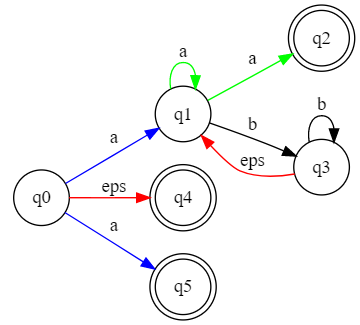
\includegraphics[width=4in, keepaspectratio]{tompson1.png}
\end{frame}%overall documentation

% overall documentation : section 
\section{Обсуждение}
%В разделе "обсуждение" можно добавлять всё что угодно по вкусу: историческую справку, какие-то интересные примеры, способы применения, связь с другими понятиями теории автоматов и т.д. Можно сделать дополнительный метакомментарий: basic documentation, добавляющую ещё какие-то простые пояснения.
\begin{frame}{Cвойства автомата Томпсона}
    \begin{itemize}
        \item Единственное начальное состояние
        \item Единственное конечное состояние
        \item Не больше двух переходов из каждого состояния
    \end{itemize}
\end{frame}
\end{document}
